% !TEX root=../../thesis.tex

\clearpage
\section{Stakeholders} % (fold)
\label{sec:back_stakeholders}
When looking at the Norwegian railway, there exists several type of users which
may be taken into consideration. On the Norwegian railway operates several
companies, who all have several positions in its organization hierarchy. Each
of these positions have different responsibilities and therefor different
interests in the system. A example of such a hierarchy is presented in
\Ref{table:user_roles}.

\begin{table}[!h]\small
	\begin{tabularx}{\textwidth}{|l|X|}
		\hline
		User type & Responsibility \\
		\hline
		Railway director & Organization director\\
		\hline
		Infrastructure director & Responsibility to facilitate that the railway traffic in Norway is safe and reliable\\
		\hline
		Area director & Responsibility to coordinate traffic within a area\\
		\hline
		Stretch director & Responsibility to coordinate traffic within certain
		stretches\\
		\hline
		Segment director & Responsibility to coordinate traffic within a segment\\
		\hline
	\end{tabularx}
\caption{User roles in the Norwegian railway network}
\label{table:user_roles}
\end{table}

This lists only relevant users from Jernbaneverket (see Section
\Vref{sub:subsection_jernbaneverket}), where the organization map is presented
online\cite{jernbaneverketOrganisasjon}\cite{jernbaneverketInfrastruktdivisjon}.
Many of the other companies which operates on the Norwegian railway system,
have a similar structure. 

When presenting information later in the thesis, the hierarchy of stakeholders of Jernbaneverket is used, which is presented in the following list.
\begin{description}
	\item [Area director] Responsible for one of six areas in which the 
	Norwegian railway is divided into.
	\item [Stretch director] Responsible for one of several stretches within 
	one area.
	\item [Segment director] Responsible a stretch of stations within one stretch.
\end{description}

\bigskip
An example of such a hierarchy is presented in the list below.

\begin{description}
	\item [Area] Midt (Middle-part of Norway).
	\item [Dovre- og Raumabanen] The northern part of the Dovre-course and the
	Rauma course.
	\item [(Dombås) - Hjerkinn] The segment of the Dovre-course which is 
	between the exit of the station on Dombås and The entrance to Hjerkinn
	station.
\end{description}

% section stakeholders (end)

\clearpage
\section{Data Sets} % (fold)
\label{sec:back_data_sets}
When performing a study of such a relatively complex system as the
Norwegian railway, there can be much information to process. Since 
Jernbaneverket stores different types of information independently, it can 
quickly become much data to take care of.\\

As Hegglund\cite[pp. 10-11]{hegglundPunklighetsdataIJernbanetraffik} describes,
Jernbaneverket measures punctuality data in two different ways and stores it 
in a punctuality database called TIOS, \Ref{fig:jernbaneverket-trafikkdata} 
shows a extract from this. They either have automatic measurements of when a 
trains passes a measure point on the eastern part of Norway, or manual 
registration the rest of the country of each passing. In 2012, there 
passed 884 passenger trains through Oslo central station alone per day\cite[p. 12]{jernbaneverketStatistikk}.
Since the passing of a measurement point by a train is being stored, large sets
of data gets accumulated over time.

\begin{figure}[!htbp]
	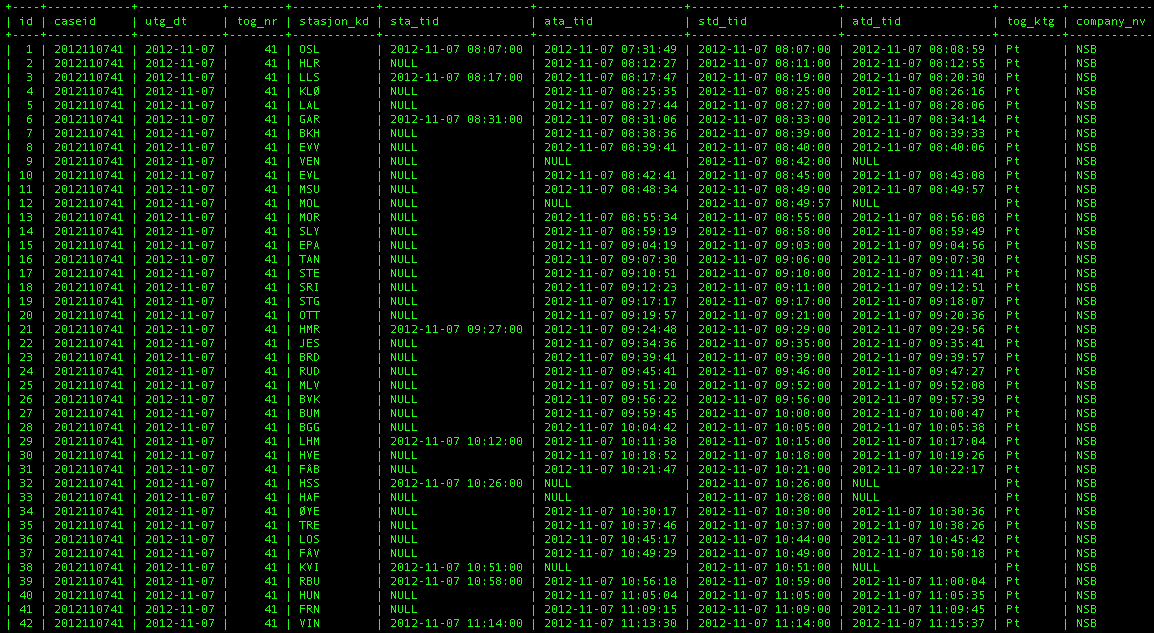
\includegraphics[width=\textwidth,center]{trafikkdata.png}
	\caption[TIOS Punctuality data]{TIOS Punctuality data \cite{sintefPresis}}
	\label{fig:jernbaneverket-trafikkdata}
\end{figure}
\pagebreak

Since this set of data stores every train that passes every measurement point,
and the corresponding time point , is is possible
to use the same set to calculate where every crossing between different trains
happens. This is is possible since one can compare the time stamps of the
passing of each station to another train.\\

When the speed restrictions is registered, they are stored in its own set of
data which is based on different forms. These data sets covers restrictions 
both due to scheduled work, such as improvement on the infrastructure, and due 
to unscheduled work, such as risk of destroyed tracks due to flooding and they 
are based on forms being filled out. This means that these sets can be quite 
large and become complex to interpret.\\

Developing a stakeholder aware method, can require different ways of analyzing
large different sets of data, and which might originate from different sources.
When developing such a method, one also needs to have a good way of limiting
the visual representation of the data to avoid filling the display with to much
information.
% section data_sets (end)

\section{Aggregation} % (fold)
\label{sec:back_aggregation}

When using the hierarchy of relevant stakeholders presented in \Ref{sec:back_stakeholders}
and the large sets of data mentioned in \Ref{sec:back_data_sets}, a
good way to limit the amount of data presented is to aggregate over the sets of
data based on hierarchy.

If one look at the example hierarchy presented in Section
\Ref{sec:back_stakeholders}, an example of such an aggregation could be as
follows. The segment director wants information of every station along the
segment. The Stretch wants summarized information from each segment, which is
aggregated from the stations. The area director wants information of every
stretch, which is aggregated from each segment.

When one is aware of the different level of details each type of stakeholder
wants, the aggregation quickly becomes a useful way of determining the
necessary data.

% section aggregation (end)
